%
%  AWAKE Data Acquisition
% ========================
%

\chapter{AWAKE Data Acquisition}
\label{Ch:DAQ}

Most of the work presented in this thesis is focused on determining the experiment parameters for Run~2 of AWAKE.
However, during the final stages of construction and commissioning of Run~1, several months were designated to help integrate AWAKE instrumentation with the CERN Control System and data logging infrastructure.
They key points of that work is presented here, and summarised in Publication~\ref{Pub:IPAC17} which was presented at IPAC in Copenhagen in 2017.

% ================================================================================================================================ %
\section{Experiment Measurements}
\label{DAQ:Experiment}

AWAKE instrumentation involves many CERN standard instruments like analogue cameras (BTVs), sensors, etc.
These are already supported by the CERN control system.
Several instruments, however, are not CERN-standard, and a subset of these again only have driver software available for the Windows operating system.
Since the CERN Control System runs on a Scientific Linux or a CERN CentOS platform, some adaptations had to be made to make these instruments available to the existing infrastructure.
They are as follows:
\begin{description}
    \item[Vapour Density Measurement:]
    The density of the Rubidium vapour is measured using a Mach-Zehnder type interferometer.
    The interferogram acquired by the interferometers is stored as a file which then needs to be imported into the logging system for post-processing.
    In post-processing, a fitting algorithm is applied to calculate the density to within $\pm0.5\%$ accuracy~\cite{oz:2016, batsch:2018}.

    \item[Laser Diagnostics:]
    The Rubidium vapour is ionised by a $4.5\unit{TW}$, $100-120\unit{fs}$ laser~\cite{gschwendtner:2016}.
    The pulse length is measured by a single shot optical auto-correlator~\cite{salin:1987}.
    This device does not produce an automatic log file of the measurement, so a special tool was written to extract the information on a trigger.
    The digital camera data is post-processed with a fitting algorithm written by the instrument operator, and the pulse width is extracted.
    The data is the written to a specially designed binary file format, which is then imported into the logging system.

    \item[Oscilloscopes:]
    Fast oscilloscopes are also used, for instance to measure real time signals from various Schottky diodes installed to measure Coherent Transition Radiation (CTR) emitted in the microwave band~\cite{braunmueller:2018}.
    Specifically, a 4-channel Tektronix oscilloscope which produces per-channel data files needed to be integrated into the data logging system.

    \item[Various Probes:]
    In addition to the above specialised instruments, a number of simple probes were needed to send single measurement values to the logging systems.
    These were treated with a flexible interface that could handle multiple data sources.
\end{description}

% ================================================================================================================================ %
\section{Data Acquisition}
\label{DAQ:DAQ}

The benefit of integrating these instruments into the existing CERN Control System at the front end is that the experiment can take direct advantage of the existing infrastructure in the other layers; that is: short and long term data logging, fixed displays and standard control system graphical user interfaces (GUIs).

\begin{figure}[hbt]
    \centering
    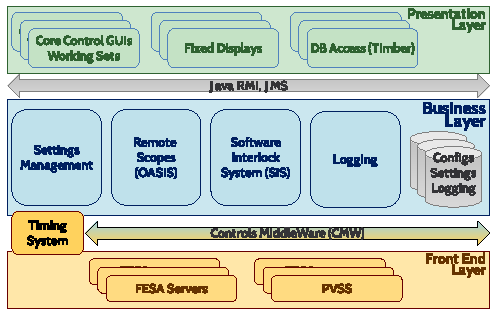
\includegraphics[width=0.85\linewidth,trim={0mm 0mm 0mm 0mm},clip]{figures/CERNControls}
    \caption{\label{Fig:DAQ:CERN}
        An overview of the CERN Control System structure.
        The system is layered, and has standardised interfaces.
        The data acquisition happens on the Front End Layer where high performance PCs and PLCs provides real time processing of raw data.
        This is then fed upstream to the data logging layer, and then made available to the displays at the top layer.
        The illustration is taken from Publication~\ref{Pub:IPAC17}, which is again recreated from~\cite{add:gorbonosov:2013}.
    }
\end{figure}

The structure of the CERN Control System is presented in Figure~\ref{Fig:DAQ:CERN}.
By integrating the new instruments at the lowest layer in the hierarchy, the standard application interfaces (APIs) between these are automatically available, significantly reducing the amount of custom code needed to be written.
This still required the instruments to be integrated at the Front End Layer, and in addition a custom tool for collecting data on an event level was written to provide single event data packages for later analysis.
This tool was named the \textit{Event Builder}, and developed by J.~Batkiewicz and R.~Gorbonosov~\cite{add:gessner:2018}.

% ================================================================================================================================ %
\subsection{Front End Software Architecture (FESA)}
\label{DAQ:FESA}

The APIs of the Control System are standardised, and this is also the case on the Front End.
The Front End Software Architecture (FESA) is a software framework originally developed at CERN.
It provides a set of tools for developers to generate large portions of the code needed to control and read instruments and control infrastructure in the main accelerators at CERN, including the LHC.
Collectively, the FESA classes provide a standard API towards the higher layers of the controls framework.

While originally developed by CERN, FESA was always intended to be usable for other experiments.
The current iteration, FESA~3, is developed in collaboration with GSI Helmholtz Centre for Heavy Ion Research in Germany, where it is used at the FAIR facility~\cite{schwinn:2010}.

% ================================================================================================================================ %
\subsection{AWAKE Integration with FESA}
\label{DAQ:Integration}

As discussed above, several of the instruments used for AWAKE only have drivers for the Windows operating system.
The straightforward solution in most of these cases were to use the file logging features available in the instrumentation software.
These generated files could then be picked up by specially prepared FESA File Reader classes accessing the Windows servers through Samba file shares.

\begin{figure}[hbt]
    \centering
    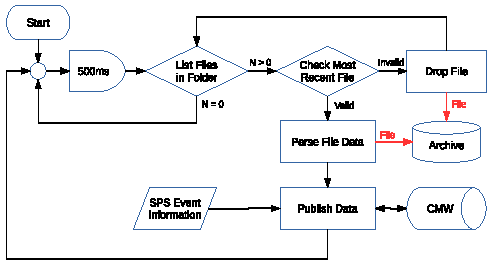
\includegraphics[width=0.85\linewidth,trim={0mm 0mm 0mm 0mm},clip]{figures/FileReader}
    \caption{\label{Fig:DAQ:Reader}
        Flow chart of the internal logic in all the FESA File Reader classes developed for AWAKE.
        Illustration taken from Publication~\ref{Pub:IPAC17}, and was originally presented at an AWAKE Technical Board meeting in 2016~\cite{add:berglyd_olsen:2016}.
    }
\end{figure}

For the laser diagnostics instrument, however, the available software did not have an automatic logging feature, so we had to write our own.
The solution was to extract data directly from the digital camera built into the instrument itself, and write to a binary file format specially designed for our purpose.
This allowed the laser diagnostics to be treated in the same way as the other instruments; with a file reader class.
Figure~\ref{Fig:DAQ:Reader} illustrates the flow used for the development of these classes.

The general flow of the file reader classes is as follows:
The class will probe for a new file every $500\unit{ms}$, building a list of files.
The list is then sorted, and the most recent file by file creation stamp is read into a buffer and parsed.
The parsing itself varies between the different classes depending on the format written by the respective instruments.
If the file is deemed to be invalid, either because it does not conform to the expected format, or it is truncated for one reason or another, the file is dropped and moved into a special folder for discarded files.
If the file is valid, the data is converted into the correct data type and published on the API.
The reader is designed such that no file is deleted, so a successfully parsed file is also moved to an archive folder.

The successfully acquired data is merged with the most recent information from the SPS accelerator, namely the information that identifies the specific proton bunch that was extracted and sent to the experiment at that given time.
When the data is published, that is made available to upstream software, a notification is sent out alerting services that subscribe the the data that a new data set is available.
If no one is listening and capturing the data, like the logging system or the Event Builder, the data is overwritten on the next successful acquisition.
The raw data is, however, still available in the archive folders in case the data flow is interrupted.

A total of four of these special FESA File Reader classes were developed as part of this thesis work.
These are all currently being used by the experiment, and being actively maintained by other members of the experiment.

% ================================================================================================================================ %
